\documentclass{article}
\usepackage{amsfonts,amsmath,amssymb,graphicx}
\usepackage[utf8]{inputenc}
\usepackage[czech]{babel}
\usepackage[numbers]{natbib}

\newtheorem{df}{Definice}
\newtheorem{veta}{Věta}

\newcommand{\0}{\vec{0}}
\newcommand{\A}{\mat A}
\newcommand{\algoritmus}[2]{\vspace{2mm}\begin{tabular}{l}
\hline
{\bf Algoritmus A\arabic{algocntr}} #1\\
\hline
#2\\
\hline
\end{tabular}\vspace{2mm}
\addtocounter{algocntr}{1}}
\newcommand{\B}{\mat B}
\newcommand{\bb}{\vec{b}}
\newcommand{\C}{\mathbb C}
\newcommand{\CC}{\mat C}
\newcommand{\cc}{\vec{c}}
\newcommand{\ee}{\vec{e}}
\newcommand{\I}{\mat I}
\newcommand{\lo}[1]{\langle #1\rangle}
\newcommand{\mat}[1]{\mathbf{#1}}
\newcommand{\N}{\mathbb N}
\newcommand{\norm}[1]{\|#1\|}
\newcommand{\pp}{\vec{p}}
\newcommand{\Q}{\mathbb Q}
\newcommand{\qq}{\vec{q}}
\newcommand{\R}{\mathbb R}
\newcommand{\range}[1]{\mathcal R(#1)}
\newcommand{\rank}{\operatorname{rank}}
\newcommand{\rr}{\vec{r}}
\newcommand{\sgn}{\operatorname{sgn}}
\renewcommand{\ss}{\vec{s}}
\newcommand{\uu}{\vec{u}}
\newcommand{\vv}{\vec{v}}
\newcommand{\ww}{\vec{w}}
\newcommand{\xx}{\vec{x}}
\newcommand{\yy}{\vec{y}}
\newcommand{\Z}{\mathbb Z}
\newcommand{\zz}{\vec{z}}

\newcounter{algocntr}
\setcounter{algocntr}{1}

\title{Aplikovaná matematika -- učební text}
\author{J. Stebel}

\begin{document}

\maketitle

\section{Úvod -- základní pojmy}

\subsection{Značení}

\begin{tabular}{ll}
$\N$ & množina přirozených čísel (1, 2, 3, \ldots)\\
$\Z$ & množina celých čísel\\
$\Q$ & množina racionálních čísel\\
$\R$ & množina reálných čísel\\
$\C$ & množina komplexních čísel\\
$A\subset B$ & $A$ je částí (podmnožinou) $B$\\
$A\cap B$ & průnik\\
$A\cup B$ & sjednocení\\
$A\setminus B$ & rozdíl množin\\
$A\times B$ & kartézský součin\\
$(a_1,\ldots,a_n)$ & uspořádaná $n$-tice\\
$(a,b)$ & otevřený interval\\
$[a,b]$ & uzavřený interval
\end{tabular}



\subsection{Relace a zobrazení}

\begin{df} {\bf Binární relace}, nebo také jen relace, mezi množinami $A$ a $B$ je libovolná podmnožina kartézského součinu $A\times B$.
\end{df}
Je-li $R$ relace mezi $A$ a $B$, pak skutečnost, že $(a,b)\in R$ zapisujeme také výrazem $aRb$.
Např. mezi množinami $A=\{\mbox{Adam, Sókratés, Karel IV.}\}$ a $B=\{\mbox{Eva, Xantippa, Marie Terezie}\}$ lze zavést relaci partnerství $P=\{\mbox{(Adam,Eva), (Sókratés,Xantippa)}\}$.
Jiným příkladem relace je uspořádání na množině $\R$, reprezentované symbolem $\le$, nebo rovnost prvků v $\R$.

\paragraph{Symetrická relace} je taková relace $R$ na množině $A$ (tedy $R\subset A\times A$), která splňuje
$$ (a,b)\in R\Leftrightarrow(b,a)\in R. $$
Příkladem symetrické relace je rovnost mezi reálnými čísly.

\paragraph{Tranzitivní relace} $R$ na množině $A$ splňuje
$$ (a,b)\in R \& (b,c)\in R\Rightarrow (a,c)\in R. $$
Relace $<$ na množině $\R$ je tranzitivní.

\paragraph{Reflexivní relace} je taková relace $R$ na množině $A$, pro kterou platí:
$$ \forall a\in A:~(a,a)\in R. $$
Relace $=$, $\le$ jsou reflexivní, $<$ není reflexivní.


\paragraph{Zobrazení} $f$ množiny $A$ do množiny $B$ je relace $f\subset A\times B$, která splňuje:
$$ \forall a\in A~\exists!b\in B:~(a,b)\in f. $$
Píšeme také $f:A\to B$, $f:a\mapsto b$, $f(a)=b$.

\paragraph{Obraz množiny} $A'$ při zobrazení $f:A\to B$ je množina
$$ f(A'):=\{f(a);~a\in A'\}. $$

\paragraph{Prosté zobrazení} má vlastnost
$$ f(a_1)=f(a_2) \Rightarrow a_1=a_2. $$

\paragraph{Inverzní zobrazení} k prostému zobrazení $f:A\to B$ je zobrazení $f^{-1}:f(A)\to A$ definované předpisem
$$ f^{-1}(b)=a \Leftrightarrow f(a)=b. $$

\paragraph{Surjektivní zobrazení} splňuje
$$ f(A)=B. $$
Někdy také říkáme, že $f$ zobrazuje $A$ \emph{na} $B$.

\paragraph{Isomorfní zobrazení,} nebo jen isomorfismus, je zobrazení, které je zároveň prosté a surjektivní.
Existuje-li mezi $A$ a $B$ isomorfismus, říkáme, že $A$ a $B$ jsou isomorfní.

Pomocí isomorfismů můžeme zavést tyto kategorie množin:
Řekneme, že množina je konečná, pokud je isomorfní s množinou $\{1,\ldots,n\}$ pro nějaké číslo $n\in\N$.
Spočetná množina je isomorfní s nějakou (ne nutně konečnou) podmnožinou $\N$.
Množina, která není konečná, se nazývá nekonečná.
Množina, která není spočetná, se nazývá nespočetná.

Např. $\N$, $\Z$, $\Q$ jsou spočetné, $\R$ je nespočetná.

\paragraph{Složené zobrazení.} Je-li $f:A\to B$ a $g:B\to C$, pak $g\circ f:A\to C$ je zobrazení složené z $f$ a $g$, které je definováno vztahem
$$ g\circ f(a) = g(f(a)). $$


\subsection{Vektorové prostory}

\begin{df}
\label{df:vekt_prostor}
Neprázdná množina $V$, na které je definováno sčítání $+:V\times V\to V$ a násobení reálným číslem $\cdot:\R\times V\to V$, se nazývá {\bf reálný vektorový prostor} (nebo také lineární prostor), jestliže pro každé $\xx, \yy, \zz\in V$ a každé $\alpha,\beta\in\R$ platí:
\begin{enumerate}
\item $\forall\xx,\yy\in V:~\xx+\yy=\yy+\xx$ \hspace{\stretch{1}}{\footnotesize(komutativita sčítání)}
\item $\forall\xx,\yy,\zz\in V:~(\xx+\yy)+\zz=\xx+(\yy+\zz)$ \hspace{\stretch{1}}{\footnotesize(asociativita sčítání)}
\item $\forall\alpha,\beta\in\R~\forall\xx\in V:~\alpha\cdot(\beta\cdot\xx)=(\alpha\beta)\cdot\xx$ \hspace{\stretch{1}}{\footnotesize(asociativita násobení)}
\item $\forall\alpha\in\R~\forall\xx,\yy\in V:~\alpha\cdot(\xx+\yy)=\alpha\cdot\xx+\alpha\cdot\yy$ \hspace{\stretch{1}}{\footnotesize(distributivita sčítání prvků z $V$)}
\item $\forall\alpha,\beta\in\R~\forall\xx\in V:~(\alpha+\beta)\cdot\xx=\alpha\cdot\xx+\beta\cdot\xx$ \hspace{\stretch{1}}{\footnotesize(distributivita sčítání čísel)}
\item $\forall\xx\in\R:~1\cdot\xx=\xx$ \hspace{\stretch{1}}{\footnotesize(vlastnost reálného čísla $1$)}
\item $\exists\0\in V ~\forall\xx\in V:~0\cdot\xx=\0$ \hspace{\stretch{1}}{\footnotesize(existence nulového prvku)}
\end{enumerate}
\end{df}

Prvky vektorového prostoru nazýváme {\bf vektory}.
Reálným číslům v kontextu násobení $\cdot:\R\times V\to V$ říkáme {\bf skaláry}.
Prvek $\0$ nazýváme {\bf nulový prvek} nebo {\bf nulový vektor}.
% 
Z axiómů uvedených v definici vektorového prostoru lze odvodit, že pro nulový prvek $\0\in V$ platí:
\begin{itemize}
\item $\forall\xx\in V$: $\xx+\0=\xx$,
\item $\forall\alpha\in\R$: $\alpha\cdot\0=\0$,
\item $\forall\xx\in V~\forall\alpha\in\R,\alpha\neq 0$: $\alpha\cdot\xx=\0\Rightarrow\xx=\0$.
\end{itemize}
% 
% 
Příklady vektorových prostorů:
\begin{itemize}
\item euklidovské prostory $\R$, $\R^2$, $\R^n$ (násobení skalárem i sčítání po složkách)
\item triviální prostor $\{\0\}$ ($\alpha\0=\0+\0=\0$)
\item prostor $\mathcal F$ reálných funkcí jedné reálné proměnné ($(\alpha f)(x):=f(\alpha x)$, $(f+g)(x):=f(x)+g(x)$)
\item prostor polynomů $\mathcal P$
\item prostor $\mathcal P_n$ polynomů stupně $\le n$
\end{itemize}

\begin{df}
Řekneme, že $W$ je {\bf podprostorem} vektorového prostoru $V$, jestliže je $W\subset V$ a množina $W$ s operacemi sčítání a násobení skalárem převzatými z $V$ je vektorový prostor.
\end{df}
Např. $\mathcal P_n$ je podprostorem $\mathcal P$ a oba jsou podprostory $\mathcal F$.

Pro zjištění, zda je nějaká množina podprostorem, není nutné ověřovat všech 7 vlastností z Definice \ref{df:vekt_prostor}.
Následující tvrzení tuto proceduru usnadňuje.
\begin{veta}
Nechť $V$ je vektorový prostor a $\emptyset\neq W\subset V$.
Pak $W$ je podprostorem $V$ právě tehdy, když platí
\begin{itemize}
\item[(i)] pro každé $\xx,\yy\in W$ je $\xx+\yy\in W$,
\item[(ii)] pro každé $\xx\in W$ a $\alpha\in\R$ je $\alpha\xx\in W$.
\end{itemize}
\end{veta}

Platí, že průnik dvou vektorových prostorů je vektorový prostor.
Sjednocení vektorových prostorů tuto vlastnost nemá.
Příklad: Jsou-li $A=\{(\alpha,0);~\alpha\in R\}$ a $B=\{(0,\beta);~\beta\in\R\}$ dva podprostory $\R^2$, pak $A\cap B=\{\0\}$ je triviální prostor.
Naproti tomu $A\cup B=\{(\alpha,\beta);~\alpha=0\mbox{ nebo }\beta=0\}$ není vektorový prostor, neboť např. $(1,0)+(0,1)=(1,1)\notin A\cup B$.

\begin{df}
Nechť $\xx_1,\xx_2,\ldots,\xx_n$ jsou prvky vektorového prostoru $V$ a $\alpha_1,\alpha_2,\ldots,\alpha_n$ jsou reálná čísla.
Vektor
$$ \alpha_1\xx_1+\alpha_2\xx_2+\ldots+\alpha_n\xx_n $$
se nazývá {\bf lineární kombinací} vektorů $\xx_1,\xx_2,\ldots,\xx_n$.
Číslům $\alpha_1,\alpha_2,\ldots,\alpha_n$ říkáme {\bf koeficienty} lineární kombinace.
\end{df}

\begin{df}
{\bf Triviální} lineární kombinace vektorů $\xx_1,\xx_2,\ldots,\xx_n$ je taková lineární kombinace, která má všechny koeficienty nulové.
{\bf Netriviální} lineární kombinace je taková, že alespoň jeden její koeficient je nenulový.
\end{df}

Poznámka: Triviální lineární kombinace je vždy rovna nulovému vektoru.

\begin{df}
Konečnou množinu vektorů $\{\xx_1,\ldots,\xx_n\}$ nazýváme {\bf lineárně závislou}, pokud existuje netriviální lineární kombinace těchto vektorů, která je rovna nulovému vektoru. Stručně říkáme, že vektory $\xx_1,\ldots,\xx_n$ jsou lineárně závislé.

Množina vektorů $\{\xx_1,\ldots,\xx_n\}$ se nazývá {\bf lineárně nezávislá}, pokud není lineárně závislá.
\end{df}

Pro 2 a více vektorů platí, že jsou lineárně závislé, právě když jeden z vektorů je roven lineární kombinaci ostatních.

Příklad: Prvky $\cos^2x$, $\sin^2x$, $\cos2x$ prostoru funkcí $\mathcal F$ jsou lineárně závislé, neboť pro libovolné $x\in\R$ platí: $\cos2x=\cos^2x+(-1)\sin^2x$.

Pojmy lineární závislost a nezávislost lze zavést také pro nekonečné množiny.
\begin{df}
Množina vektorů $M$ se nazývá {\bf lineárně závislá}, pokud v ní existuje \emph{konečná} podmnožina, která je lineárně závislá.

Množina vektorů $M$ se nazývá {\bf lineárně nezávislá}, pokud není lineárně závislá.
\end{df}
Příkladem lineárně nezávislé množiny v $\mathcal P$ je množina $\{1,x,x^2,x^3,x^4,\ldots\}$.

\begin{df}
{\bf Lineární obal} konečné množiny $\{\xx_1,\ldots,\xx_n\}$ je množina všech lineárních kombinací těchto vektorů.
Lineární obal nekonečné množiny $M$ je sjednocení lineárních obalů všech konečných podmnožin množiny $M$.
\end{df}

Lineární obal množiny $\{\xx_1,\ldots,\xx_n\}$ značíme $\lo{\xx_1,\ldots,\xx_n}$.
Lineární obal množiny $M$ značíme $\lo{M}$.
% 
% \begin{veta}
% Nechť $V$ je vektorový prostor a $M,N$ jsou jeho podmnožiny. Pak platí:
% \begin{enumerate}
% \item $M\subset \lo{M}$.
% \item $\lo M = \lo{\lo M}$.
% \item Je-li $\zz\in\lo M$, pak $\lo M = \lo{M\cup\{\zz\}}$.
% \item Je-li $M\subset N$, pak $\lo M\subset\lo N$.
% \end{enumerate}
% \end{veta}
% 
% \begin{veta}
% Nechť $V$ je vektorový prostor a $M\subset V$.
% Množina $M$ je podprostorem $V$, právě když $M=\lo M$.
% \end{veta}
% 
% Lineární obal jakékoliv množiny je vektorový prostor.
% 
% \begin{veta}
Je-li $M$ podmnožina vektorového prostoru $V$, pak $\lo M$ je nej\-men\-ší vektorový prostor obsahující množinu $M$.
% \end{veta}


\begin{df}
{\bf Báze} vektorového prostoru $V$ je množina $B\subset V$, pro kterou platí:
\begin{itemize}
\item[(i)] $B$ je lineárně nezávislá,
\item[(ii)] $\lo B=V$.
\end{itemize}
\end{df}

\begin{veta}
% \begin{enumerate}
V každém netriviálním vektorovém prostoru existuje báze.
Jsou-li $B_1$ a $B_2$ dvě báze vektorového prostoru $V$, pak jsou obě nekonečné nebo mají stejný počet prvků.
% \end{enumerate}
\end{veta}

% \begin{veta}
% Nechť $\xx_1,\ldots,\xx_n$ jsou prvky vektorového prostoru $V$, z nichž alespoň jeden je nenulový.
% Pak z nich lze vybrat prvky $\xx_{s_1}, \xx_{s_2},\ldots,\xx_{s_k}$, kde $1\le s_1<s_2<\ldots<s_k\le n$, takové, že
% \begin{itemize}
% \item[(i)] $\xx_{s_1},\ldots,\xx_{s_k}$ jsou lineárně nezávislé,
% \item[(ii)] $\lo{\xx_{s_1},\ldots,\xx_{s_k}}=\lo{\xx_1,\ldots,\xx_n}$.
% \end{itemize}
% \end{veta}

\begin{veta}
Nechť vektory $\xx_1,\ldots,\xx_n$ tvoří bázi vektorového prostoru $V$.
Je-li $\xx\in V$ libovolný vektor, pak existuje právě jedna uspořádaná $n$-tice čísel $(c_1,\ldots,c_n)$ taková, že
$$ \xx = c_1\xx_1+\ldots+c_n\xx_n. $$
\end{veta}

\begin{df}
Čísla $c_1,\ldots,c_n$ z předchozí věty se nazývají {\bf souřadnice} vektoru $\xx$ v bázi $\xx_1,\ldots,\xx_n$.
\end{df}

\begin{df}
{\bf Dimenze} vektorového prostoru $V$ je počet prvků báze tohoto prostoru.
Označujeme ji symbolem $\dim V$.
Speciální případy:
\begin{itemize}
\item Triviální prostor má dimenzi 0.
\item Pokud je báze prostoru nekonečná, pak klademe $\dim V=\infty$.
\end{itemize}
\end{df}
% 
% \begin{veta}
Je-li $V$ vektorový prostor a $M$ je podprostor $V$, pak $\dim M \le\dim V$.
% \end{veta}

\begin{veta}
Nechť $V$ je vektorový prostor, jehož dimenze je $\dim V=n$ a $M=\{\xx_1,\ldots,\xx_m\}$.
Pak platí:
\begin{enumerate}
\item Je-li $M$ lineárně nezávislá, pak $m\le n$.
\item Je-li $m>n$, pak $M$ je lineárně závislá.
\item Nechť $m=n$. Pak $M$ je lineárně nezávislá, právě když $\lo M=V$.
\end{enumerate}
\end{veta}



\subsection{Lineární zobrazení, matice}

\begin{df}
Zobrazení $f$ vektorového prostoru $V$ do vektorového prostoru $W$ se nazývá {\bf lineární}, jestliže pro každé $\alpha\in\R$ a $\xx,\yy\in V$ platí:
$$ f(\alpha\xx+\yy)=\alpha f(\xx) + f(\yy). $$
{\bf Jádrem} tohoto zobrazení rozumíme množinu
$$ \ker f:=\{\xx\in V;~f(\xx)=\0\}. $$
{\bf Obraz} $f$ je množina
$$ \range f :=f(V). $$
\end{df}
Lineární zobrazení $f$ je prosté právě tehdy, když $\ker f=\{\0\}$.
\begin{veta}
Jsou-li vektory $\xx_1,\ldots,\xx_k$ lineárně závislé, pak jsou lineárně závislé také vektory $f(\xx_1),\ldots,f(\xx_k)$.
Pokud je navíc $f$ prosté, pak platí i obrácené tvrzení, tedy
$$ \xx_1,\ldots,\xx_k \mbox{ jsou lineárně závislé }\Leftrightarrow f(\xx_1),\ldots,f(\xx_k)\mbox{ jsou lineárně závislé}. $$
\end{veta}


\begin{df}
{\bf (Reálná) matice} typu $(m,n)$ je symbol
$$ \A=\begin{pmatrix}a_{1,1} & a_{1,2} & \ldots & a_{1,n}\\a_{2,1} & a_{2,2} & \ldots & a_{2,n}\\&&\vdots&\\a_{m,1} & a_{m,2} & \ldots & a_{m,n}\end{pmatrix} = (a_{ij})_{i=1,\ldots,m}^{j=1,\ldots,n}, $$
kde pro $i=1,\ldots,m$ a $j=1,\ldots,n$ jsou $a_{ij}$ reálná čísla (nazývají se {\bf prvky} matice $\A$).
% 
% Pro $i=1,\ldots,m$ nazýváme $n$-tici čísel $(a_{i,1},a_{i,2},\ldots,a_{i,n})$ $i$-tým {\bf řádkem} matice $\A$.
% 
% Pro $j=1,\ldots,n$ nazýváme $m$-tici čísel $\begin{pmatrix}a_{1,j}\\a_{2,j}\\\vdots\\a_{m,j}\end{pmatrix}$ $j$-tým {\bf sloupcem} matice $\A$.
\end{df}
Množinu všech matic typu $(m,n)$ budeme značit $\R^{m\times n}$.
Definujeme-li sčítání matic a násobení matic reálným číslem po složkách, pak množina $\R^{m\times n}$ je vektorový prostor.

\begin{df}
Řekneme, že $\B\in\R^{n\times m}$ je {\bf transponovaná matice} k matici $\A\in\R^{m\times n}$, jestliže
$$ \forall i=1,\ldots,m~\forall j=1,\ldots,n:~a_{ij}=b_{ji}. $$
Píšeme také $\B=\A^\top$.
\end{df}
\begin{df}
Řekneme, že matice $\A$ je {\bf symetrická}, jestliže $\A=\A^\top$.
\end{df}
% 
Součin matic $\A\in\R^{m\times n}$ a $\B\in\R^{n\times p}$ je matice $\mat C\in\R^{m\times p}$, jejíž složky splňují:
$$ c_{ij} = \sum_{k=1}^n a_{ik}b_{kj},~i=1,\ldots,m,~j=1,\ldots,p. $$
Násobení matic není komutativní, tj. obecně $\A\B\neq\B\A$.
Pro matice vhodných typů (takových, aby je šlo násobit), platí:
$$ \begin{aligned}
&\A(\B\mat C)=(\A\B)\mat C,\\
&(\A+\B)\mat C=\A\mat C+\B\mat C,\\
&(\alpha\A)\B=\A(\alpha\B)=\alpha(\A\B),~\alpha\in\R.
\end{aligned} $$
\begin{df}
Čtvercovou matici $\I=(e_{i,j})\in\R^{n\times n}$ nazýváme {\bf jednotkovou maticí}, jestliže pro její prvky platí: $e_{i,j}=0$ pro $i\neq j$ a $e_{i,j}=1$ pro $i=j$.
\end{df}
\begin{df}
Řekneme, že $\B\in\R^{n\times n}$ je {\bf inverzní matice} k matici $\A\in\R^{n\times n}$, pokud $\A\B=\B\A=\I$.
Tuto matici značíme symbolem $\B=\A^{-1}$.
Pokud existuje $\A^{-1}$, pak matici $\A$ nazýváme {\bf regulární}. V opačném případě se $\A$ nazývá {\bf singulární} matice.
\end{df}

\begin{df}
{\bf Hodnost matice} $\A$ je počet lineárně nezávislých řádků v této matici.
Značíme ji $\rank\A$.
\end{df}
Platí také, že hodnost je rovna počtu lineárně nezávislých sloupců, tedy $\rank\A^\top=\rank\A$.
Matice $\A\in\R^{n\times n}$ je regulární právě tehdy, když platí: $\rank\A=n$.


\begin{df}
{\bf Permutace} $n$ prvků je uspořádaná $n$-tice čísel $1,2,\ldots,n$ taková, že žádné číslo se v ní neopakuje.
\end{df}
Poznámka: Počet různých permutací $n$ prvků je roven číslu $n!$.

\begin{df}
Nechť $(i_1,i_2,\ldots,i_n)$ je permutace $n$ prvků.
{\bf Počet inverzí} této permutace je počet takových dvojic $(i_k,i_l)$, pro které platí $i_k>i_l$, a přitom $k<l$.
\end{df}

\begin{df}
Pro každou permutaci $\pi=(i_1,\ldots,i_n)$ definujeme její {\bf znaménko} $\sgn\pi$ takto:
$$ \sgn\pi = \begin{cases}+1 & \mbox{má-li $\pi$ sudý počet inverzí}\\-1 & \mbox{má-li $\pi$ lichý počet inverzí}\end{cases} $$
\end{df}
Prohozením dvou prvků v permutaci způsobí změnu jejího znaménka.

\begin{df}
Nechť $\A=(a_{i,j})\in\R^{n\times n}$. {\bf Determinant} matice $\A$ je číslo
$$ \det\A=\sum_{\pi=(i_1,i_2,\ldots,i_n)}(\sgn\pi) a_{1,i_1} a_{2,i_2} \cdots a_{n,i_n}. $$
V uvedeném vzorci se sčítá přes všechny permutace $n$ prvků, tj. jedná se o $n!$ sčítanců.
\end{df}


\begin{veta}
Nechť $\A,\B\in\R^{n\times n}$.
Pak platí:
\begin{enumerate}
\item $\det\A=0$ právě tehdy, když $\A$ je singulární,
\item $\det\A^\top=\det\A$,
\item $\det(\A\B)=(\det\A)(\det\B)$,
\item $\det(\A^{-1})=1/\det\A$.
\item Jestliže se $\B$ liší od $\A$ jen prohozením dvojice řídků, pak $\det\B=-\det\A$.
\item Jestliže matice $\A$ má dva stejné řádky, pak $\det\A=0$.
\end{enumerate}
\end{veta}

\begin{df}
Číslo $\lambda\in\C$ se nazývá {\bf vlastním číslem} matice $\A\in\C^{n\times n}$, jestliže existuje nenulový vektor $\uu\in\C^n$ takový, že
$$ \A\uu=\lambda\uu. $$
Vektor $\uu$ se pak nazývá {\bf vlastní vektor} matice $\A$ příslušný vlastnímu číslu $\lambda$.
Množina všech vlastních čísel $A$ se nazývá {\bf spektrum} matice $\A$ a značí se $\sigma(\A)$.
\end{df}
Číslo $\lambda$ je vlastním číslem $\A$ právě tehdy, má-li soustava $(\A-\lambda\I)$ netriviální řešení, tj. právě tehdy, je-li $\A-\lambda\I$ singulární, což je ekvivalentní podmínce $\det(\lambda\I-\A)=0$.
Polynom $\chi_\A(\lambda):=\det(\lambda\I-\A)$ se nazývá {\bf charakteristický polynom} matice $\A$.
Číslo $\lambda$ je tedy vlastním číslem $\A$, je-li kořenem $\chi_\A$.
Poznamenejme, že polynom s reálnými koeficienty může mít komplexní kořeny, a reálná matice může proto mít komplexní vlastní čísla.
Je-li ovšem reálná matice symetrická, pak jsou všechna její vlastní čísla reálná.




% matice zobrazení
% matice složeného, inverzního zobrazení
% norma, číslo podmíněnosti


\subsection{Soustava lineárních rovnic}

V dalším ztotožníme vektory z $\R^n$ s maticemi typu $(n,1)$, tj. $\vec a\in\R^n$ znamená totéž jako $\vec a\in\R^{n\times 1}$.

\begin{df}
Nechť $\A\in\R^{m\times n}$, $\xx=\begin{pmatrix}x_1\\\vdots\\x_n\end{pmatrix}\in\R^{n}$ a $\vec b=\begin{pmatrix}b_1\\\vdots\\b_m\end{pmatrix}\in\R^{m}$.
Pak maticovou rovnost
$$ \A\xx=\vec b $$
mazýváme {\bf soustavou $m$ lineárních rovnic o $n$ neznámých}.
Matici $\A$ nazýváme {\bf maticí soustavy} a vektor $\vec b$ nazýváme {\bf vektorem pravých stran}.
Připíšeme-li k matici soustavy do dalšího sloupce vektor $\vec b$ (pro přehlednost oddělený svislou čarou), dostáváme matici $(\A|\vec b)\in\R^{m\times(n+1)}$, kterou nazýváme {\bf rozšířenou maticí soustavy}.
\end{df}

  
\begin{df}
{\bf Řešením} soustavy $\A\xx=\vec b$ je takový vektor $\vec a=(\alpha_1,\ldots,\alpha_n)\in\R^n$, pro který platí: Dosadíme-li hodnoty $\alpha_i$ za symboly $x_i$, pak je splněna požadovaná maticová rovnost, tj.
$$ \A \begin{pmatrix}\alpha_1\\\vdots\\\alpha_n\end{pmatrix}=\begin{pmatrix}b_1\\\vdots\\b_m\end{pmatrix}. $$
{\bf Řešit soustavu} $\A\xx=\vec b$ znamená nalézt všechna její řešení, tj. nalézt podmnožinu $\R^n$ všech řešení této soustavy.
\end{df}

\begin{veta}[Frobeniova]
Soustava $\A\xx=\vec b$ má řešení právě tehdy, když
$$ \rank{\A}=\rank{\A|\vec b}, $$
tj. když hodnost matice soustavy se rovná hodnosti rozšířené matice soustavy.
\end{veta}

  
\begin{df}
Nechť $\A\xx=\vec b$ je soustava $m$ lineárních rovnice o $n$ neznámých a $\mat C\xx=\vec d$ je soustava $k$ lineárních rovnic o stejném počtu $n$ neznámých.
Říkáme, že tyto soustavy jsou {\bf ekvivalentní}, pokud obě soustavy mají stejné množiny řešení.
\end{df}

\begin{veta}
Ke každé soustavě $\A\xx=\vec b$ lze nalézt ekvivalentní soustavu $\mat C\xx=\vec d$, jejíž matice $\mat C$ je horní trojúhelníková.
\end{veta}
  
\begin{df}
Existuje-li v matici $\vec b$ aspoň jeden prvek nenulový, říkáme, že soustava $\A\xx=\vec b$ je {\bf nehomogenní}.
Jsou-li všechny prvky v matici $\vec b$ nulové, nazýváme soustavu rovnic {\bf homogenní} a zapisujeme ji takto:
$$ \A\xx=\0. $$
\end{df}

\begin{veta}
Množina všech řešení homogenní soustavy $\A\xx=\0$ s $n$ neznámými tvoří podprostor vektorového prostoru $\R^n$.
\end{veta}
  
\begin{veta}
Nechť $\A\xx=\0$ je homogenní soustava lineárních rovnic o $n$ neznámých.
Označme $k:=n-\rank\A$.
Pak existuje $k$ lineárně nezávislých vektorů $\uu_1,\ldots,\uu_k\in\R^n$ takových, že pro množinu $M_0$ všech řešení soustavy $\A\xx=\0$ platí:
$$ M_0=\lo{\uu_1,\ldots,\uu_k}. $$
Vektory $\uu_1,\ldots,\uu_k$ tvoří jednu z možných bází vektorového prostoru všech řešení $M_0$.
\end{veta}

Důsledek: Je-li $M_0$ vektorový prostor všech řešení homogenní soustavy lineárních rovnic $\A\xx=\0$ s $n$ neznámými, pak $\dim M_0=n-\rank\A$.
  
\begin{df}
Libovolné řešení $\vec v\in\R^n$ nehomogenní soustavy lineárních rovnic $\A\xx=\bb$ o $n$ neznámých se nazývá {\bf partikulární řešení} této soustavy.

Pokud zaměníme matici $\bb$ za nulovou matici stejného typu, dostáváme homogenní soustavu $\A\xx=\0$, kterou nazýváme {\bf přidruženou homogenní soustavou} k soustavě $\A\xx=\bb$.
\end{df}
  
\begin{veta}
\begin{enumerate}
\item Nechť $\vec v$ je partikulární řešení nehomogenní soustavy $\A\xx=\bb$ a $\uu$ je libovolné řešení přidružené homogenní soustavy $\A\xx=\0$.
Pak $\vec v+\uu$ je také řešením soustavy $\A\xx=\bb$.
\item Nechť $\vec v$ a $\vec w$ jsou dvě partikulární řešení nehomogenní soustavy $\A\xx=\bb$.
Pak $\vec v-\vec w$ je řešením přidružené homogenní soustavy $\A\xx=\0$.
\end{enumerate}
\end{veta}
  
\begin{veta}
Nechť $\vec v$ je partikulární řešení soustavy $\A\xx=\bb$ a $M_0$ je vektorový prostor všech řešení přidružené homogenní soustavy $\A\xx=\0$.
Pak pro množinu $M$ všech řešení soustavy $\A\xx=\bb$ platí:
$$ M=\{\vec v+\uu;~\uu\in M_0\}. $$
\end{veta}
  
\begin{veta}[Cramerovo pravidlo]
Nechť $\A$ je čtvercová regulární matice.
Pak pro $i$-tou složku řešení soustavy $\A\xx=\bb$ platí:
$$ \alpha_i = \frac{\det\B_i}{\det\A}, $$
kde matice $\B_i$ je shodná s $\A$ až na $i$-tý sloupec, který je zaměněn za sloupec pravých stran.
\end{veta}



\section{Iterační metody řešení soustav lineárních rovnic}

V této kapitole se budeme zabývat numerickým řešením soustavy
$$ \A\xx=\bb. $$
Předpokládáme, že čtenáři je známa Gaussova eliminační metoda, která je pří\-kla\-dem tzv. přímých metod.
Její výhodou je univerzálnost --- metoda vyřeší v přesné aritmetice soustavu s libovolnou regulární maticí.
Nevýhodou je její neefektivita pro velké matice a také to, že v průběhu výpočtu nemá uživatel žádnou informaci o výsledku.
Pro úlohy s velkou řídkou maticí $\A$, se kterými se setkáváme v mnoha praktických problémech, nebo pro úlohy, kde matice není dána explicitně nebo je drahé ji sestavit, může být výhodou použít iterační metody.
Tyto metody v zásadě používají jen násobení matic a v průběhu výpočtu postupně vylepšují aproximaci přesného řešení.
Konvergence iteračního procesu může být asymptotická nebo v konečném počtu iterací.

Pro detaily ohledně odvození a dalších vlastností iteračních metod odkazujeme na knihu \cite{analyza_metod_maticove_vyp}.



\subsection{Klasické iterační metody}

Klasické iterační metody jsou založeny na štěpení matice soustavy $\A = \mat M + \mat N$ takovém, že matice $\mat M$ je regulární a snadno invertovatelná a $\mat M$ a $\mat N$ jsou zvoleny nějakým vhodným způsobem.
Dosazením tohoto štěpení do vztahu $\mat A\xx = \bb$ dostáváme $(\mat M + \mat N)\xx = \bb$ a odtud
$$ \xx = \mat M^{-1}(\bb - \mat N\xx) = \mat M^{-1}(\bb + \mat M\xx - \mat A\xx) = \xx + \mat M^{-1}(\bb - \mat A\xx). $$
Je-li dána počáteční aproximace řešení $\xx_0$, můžeme definovat iterační proces následovně:
$$ \xx_k = \xx_{k-1} + \mat M^{-1} (\bb - \mat A\xx_{k-1} )
= (\I - \mat M^{-1}\mat A)\xx_{k-1} + \mat M^{-1}\bb. $$
Lze ukázat, že pro chybu aproximace platí odhad
$$ \frac{\norm{\xx-\xx_k}}{\norm{\xx-\xx_0}} \le \norm{(\I-\mat M^{-1}\A)^k} \le \norm{\I-\mat M^{-1}\A}^k, $$
přičemž pro velká $k$ je $\norm{(\I-\mat M^{-1}\A)^k}\approx\rho(\I-\mat M^{-1}\A)^k$ (symbolem $\rho(\A)$ značíme tzv. spektrální poloměr, který je definován jako $\max\{|\lambda|;~\lambda\in\sigma(\A)\}$).
Vidíme tedy, že metody konvergují k přesnému řešení, pokud $\rho(\I-\mat M^{-1}\A)<1$.
I v případě, že tato podmínka je splněna, však může být $\norm{\I-\mat M^{-1}\A}^k>1$ a dochází pak k tzv. přechodovému jevu, kdy chyba aproximace nejprve roste a teprve pak začne klesat (viz obr. \ref{fig:prechod}).
\begin{figure}
\centering
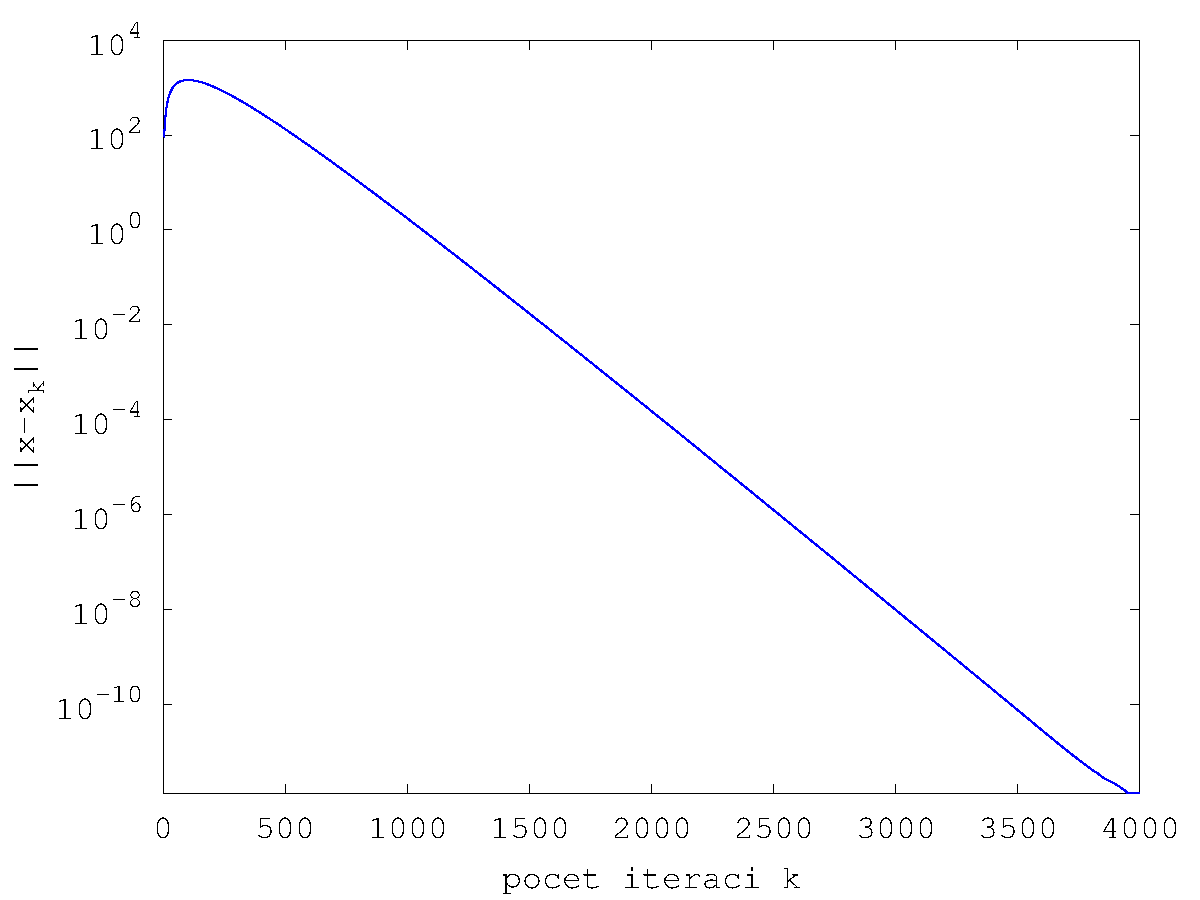
\includegraphics[width=6cm]{img/prechod}
\caption{Přechodový jev u klasické iterační metody.}
\label{fig:prechod}
\end{figure}


\paragraph{Příklady klasických iteračních metod.}
Následující metody jsou založeny na štěpení $\A=\mat D-\mat L-\mat U$, kde $\mat D$ je hlavní diagonála, $-\mat L$ je striktně dolní trojúhelník matice $\A$ a $-\mat U$ je striktně horní trojúhelník.
Z rovnice
$$ (\mat D-\mat L-\mat U)\xx=\bb $$
pak lze odvodit jednotlivé metody.

{\bf Jacobiova metoda} je definována iterací
$$ \mat D\xx_k=\mat L\xx_{k-1} + \mat U\xx_{k-1} + \bb. $$
Rozepíšeme-li tento vzorec po složkách ($x_i^k$ značí $i$-tou složku vektoru $\xx_k$), dostaneme pro $i=1,\ldots,n$:
$$ x_i^k = \frac1{a_{ii}}\left(b_i-\sum_{j=1,j\neq i}^n a_{ij}x_j^{k-1}\right). $$
Nevýhodou této metody může být, že v průběhu výpočtu je třeba uchovávat dvě posobě jdoucí aproximace řešení $\xx_k$, $\xx_{k-1}$.
Metoda {\bf Gauss-Seidelova} se od předchozí liší v tom, že ihned využívá již spočtené složky vektoru $\xx_k$, tj. po složkách počítá
$$ x_i^k = \frac1{a_{ii}}\left(b_i-\sum_{j=1}^{i-1} a_{ij}x_j^k-\sum_{j=i+1}^n a_{ij}x_j^{k-1}\right). $$
Spočtené složky aproximace řešení je tedy možné ihned přepisovat.
Maticově lze tuto iteraci zapsat jako
$$ \mat D\xx_k=\mat L\xx_k+\mat U\xx_{k-1}+\bb. $$
Z Gauss-Seidelovy metody je odvozena {\bf Superrelaxační metoda} (SOR, successive over-relaxation).
Pracuje s relaxačním parametrem $\omega\in[0,2]$ a je definována vztahem
$$ \mat D\xx_k = \omega(\mat L\xx_k+\mat U\xx_{k-1}+\bb) + (1-\omega)\mat D\xx_{k-1}, $$
tj. kombinuje Gauss-Seidelovu metodu s předchozí iterací.






\subsection{Metody Krylovových podprostorů}

Důležitá třída iteračních metod je založena na myšlence projektovat soustavu $\A\xx=\bb$ na posloupnost tzv. Krylovových prostorů a tím získávat postupně aproximace řešení.
\begin{df}
Nechť $\A\in\R^{n\times n}$, $\vv\in\R^n$ a $k\le n$.
$k$-tým Krylovovým prostorem nazýváme podprostor
$$ \mathcal K_k(\A,\vv):=\lo{\vv,\A\vv,\A^2\vv,\ldots,\A^{k-1}\vv}. $$
\end{df}
Metody, které zmíníme v následující části, mají společnou vlastnost tzv. projekčních metod, tj. hledají aproximace ve tvaru
$$ \xx_k\in \xx_0 + \mathcal S_k, \quad \rr_k\perp\mathcal C_k, $$
kde $\rr_k:=\bb-\A\xx_k$ je tzv. reziduum a $\mathcal S_k$ a $\mathcal C_k$ jsou vhodné podprostory.
Prostor $\mathcal S_k$ je obvykle roven Krylovovu podprostoru $\mathcal K_k(\A,\rr_0)$, ale jsou možné i jiné volby, např. $\A\mathcal K_k(\A,\rr_0)$.
Volbou prostoru $\mathcal C_k$ lze docílit optimality aproximace řešení v tom smyslu, že chyba aproximace $\xx-\xx_k$ je v nějaké normě minimální.
Pokud dimenze podprostorů $\mathcal S_k$, $\mathcal C_k$ roste, pak pro $k=n$ dostáváme $\mathcal C_n=\R^n$ a z podmínky $\rr_k\perp\mathcal\R^n$ plyne $\rr_n=\0$, tedy $\xx_n=\xx$ je přesné řešení.
Jinak řečeno, rostou-li dimenze prostorů $\mathcal S_k$, $\mathcal C_k$, pak projekční metody najdou řešení systému $\A\xx=\bb$ nejvýše v $n$ krocích.


\subsubsection{Metoda sdružených gradientů (CG)}
\label{sec:cg}

Tato metoda (stručně ji budeme označovat symbolem CG --- z anglického \emph{Conjugate gradients}) je určena pro symetrické pozitivně definitní matice.
\begin{df}
Matice $\A\in\R^{n\times n}$ je pozitivně definitní, pokud pro každý nenulový vektor $\xx\in\R^n$ platí:
$$ \A\xx\cdot\xx>0. $$
Výraz
$$ \norm{\xx}_\A:=\sqrt{\xx\cdot\A\xx} $$
se nazývá energetická norma nebo také $\A$-norma.
Řekneme, že vektory $\uu,\vv\in\R^n$ jsou navzájem $\A$-ortogonální, jestliže
$$ \uu\cdot\A\vv=0. $$
\end{df}
Aproximace řešení je v metodě CG konstruována podle vzorce
$$ \xx_k:=\xx_{k-1}+\gamma_{k-1}\pp_{k-1}, $$
kde $\pp_{k-1}$ je směrový vektor a $\gamma_{k-1}$ je délka kroku.
Tyto parametry se určí následujícím způsobem:
\begin{itemize}
\item $\pp_k$ volíme ve tvaru $\pp_k:=\rr_k+\delta_k\pp_{k-1}$ tak, aby byl $\A$-ortogonální na $\pp_{k-1}$, tj. $\pp_k\cdot\A\pp_{k-1}=0$. Toho docílíme pro
$$ \delta_k:=\frac{\rr_k\cdot\rr_k}{\rr_{k-1}\cdot\rr_{k-1}}. $$
\item $\gamma_{k-1}$ volíme takové, aby byla minimální energetická norma $\norm{\xx-\xx_k}_\A$. To nastane právě tehdy, když
$$ \gamma_{k-1}:=\frac{\rr_{k-1}\cdot\rr_{k-1}}{\pp_{k-1}\cdot\A\pp_{k-1}}. $$
\end{itemize}
Na základě předchozích vztahů lze ukázatm že CG patří mezi Krylovovské metody, neboť platí:
$$ \xx_k\in\xx_0+\mathcal K_k(\A,\rr_0),\quad \rr_k\perp\mathcal K_k(\A,\rr_0). $$
Na metodu sdružených gradientů lze také nahlížet jako na metodu, která hledá mi\-ni\-mum kvadratického funkcionálu $\frac12\xx\cdot\A\xx-\xx\cdot\bb$.
Následující algoritmus reprezentuje standardní implementaci metody CG.

\algoritmus{Metoda sdružených gradientů}{
{\bf input} $\A$, $\bb$, $\xx_0$\\
$\rr_0:=\bb-\A\xx_0$\\
$\pp_0:=\rr_0$\\
{\bf for }$k=1,2,\ldots$\\
$\quad \gamma_{k-1}:=\frac{\rr_{k-1}\cdot\rr_{k-1}}{\pp_{k-1}\cdot\A\pp_{k-1}}$\\
$\quad \xx_k:=\xx_{k-1}+\gamma_{k-1}\pp_{k-1}$\\
$\quad \rr_k:=\rr_{k-1}-\gamma_{k-1}\A\pp_{k-1}$\\
$\quad \delta_k:=\frac{\rr_k\cdot\rr_k}{\rr_{k-1}\cdot\rr_{k-1}}$\\
$\quad \pp_k:=\rr_k+\delta_k\pp_{k-1}$\\
{\bf end}
}

Vidíme, že v každé iteraci je třeba provést 1 násobení matice $\A$ s vektorem a v průběhu výpočtu je třeba uchovávat pouze 4 vektory.
Metoda CG je tedy velmi efektivní zejména pro velké řídké matice.
Je-li matice symetrická pozitivně definitní, pak v přesné aritmetice algoritmus nalezne řešení nejvýše po $n$ iteracích.
V praxi ovšem kvůli zaokrouhlovacím chybám dochází ke ztrátě $\A$-ortogonality vektorů $\{\pp_k\}$ (resp. ortogonality vektorů $\{\rr_k\}$), což způsobuje zpoždění konvergence, tedy že i po $n$ krocích je $\xx_n\neq\xx$.
Tento nedostatek se někdy odstraňuje tak, že se vektor $\rr_k$ ortogonalizuje proti všem předchozím $\{\rr_i\}_{i=0}^{k-1}$ a proces ortogonalizace se zopakuje vícekrát (obvykle stačí dvakrát).

Nyní si uvedeme, co je známo o rychlosti konvergence metody CG.
K tomu potřebujeme znát pojem \emph{číslo podmíněnosti}.
\begin{df}
Nechť $\A$ je symetrická pozitivně definitní matice.
Číslo podmíněnosti matice $\A$ je definováno předpisem
$$ \varkappa(\A):=\frac{\lambda_{max}(\A)}{\lambda_{min}(\A)}, $$
kde $\lambda_{max}(\A)$, $\lambda_{min}(\A)$ značí největší, resp. nejmenší vlastní číslo matice $\A$.
\end{df}
Označíme-li $\ee_k:=\xx_k-\xx$ chybu $k$-té aproximace řešení, pak platí následující odhad chyby:
$$ \frac{\norm{\ee_k}_\A}{\norm{\ee_0}_\A} \le 2\left(\frac{\sqrt{\varkappa(\A)}-1}{\sqrt{\varkappa(\A)}+1}\right)^k. $$
Všimněme si, že číslo v závorce v předchozí nerovnosti je vždy menší než $1$.
Pokud je $\varkappa(\A)$ blízké $1$, pak odhad chyby říká, že chyba klesá velmi rychle.
Pro špatně podmíněné matice (tj. je-li $\varkappa(\A)$ velké) je číslo v závorce blízké jedné a odhad často nadhodnocuje skutečnou velikost $\A$-normy chyby.
Špatná podmíněnost matice přesto může mít za následek pomalou konvergenci metody.
Tuto skutečnost lze řešit pomocí tzv. předpodmínění, které spočívá v tom, že původní soustava $\A\xx=\bb$ se nahradí ekvivalentní soustavou $\hat\A\hat\xx=\hat\bb$ s maticí $\hat\A$, která má menší číslo podmíněnosti než $\A$.



% sdružené gradienty - zastavovací kritéria, počáteční aproximace
\subsubsection{Zobecněná metoda minimálních reziduí (GMRES)}

Metodu GMRES (generalized minimal residual method) lze charakterizovat ve smyslu projekčních metod pomocí vztahů
$$ \xx_k\in\xx_0+\mathcal K_k(\A,\rr_0),\quad \rr_k\perp\A\mathcal K_k(\A,\rr_0). $$
Jak napovídá název, její vlastností je, že v každé iteraci minimalizuje normu rezidua $\norm{\rr_k}$.
To vede na úlohu nejmenších čtverců, jejíž efektivní implementace je poměrně technicky obtížná.
Proto zde její algoritmus neuvádíme.
Nepříjemnou vlastností metody GMRES je, že produkuje posloupnost ortogonálních vektorů $\{\vv_k\}$, které je třeba uchovávat, (říkáme, že metoda generuje dlouhé rekurence) a to klade vysoké nároky na paměť.
Za tuto cenu ovšem metoda dokáže řešit soustavu s libovolnou regulární maticí.

% \algoritmus{Zobecněná metoda minimálních reziduí (GMRES)}{
% {\bf input} $\A$, $\bb$, $\xx_0$\\
% $\rr_0:=\bb-\A\xx_0$\\
% $\vv_1:=\rr_0/\norm{\rr_0}$\\
% {\bf for }$k=1,2,\ldots$\\
% \quad$\ww:=\A\vv_k$\\
% \quad{\bf for }$i=1,\ldots,k$\\
% \qquad $h_{i,k}:=\vv_i\cdot\ww$\\
% \qquad $\ww:=\ww- h_{i,k}\vv_i$\\
% \quad{\bf end}\\
% \quad$h_{k+1,k}:=\norm{\ww}$\\
% 
% {\bf end}
% }

Stejně jako u metody CG, vlivem zaokrouhlovacích chyb dochází ke zpomalení konvergence kvůli ztrátě ortogonality systému $\{\vv_k\}$.
I u GMRES tedy obvykle provádíme vícenásobnou ortogonalizaci.
Problém s paměťovou náročností se obvykle řeší pomocí tzv. restartu --- program uchovává místo celé posloupnosti jen posledních $m$ vektorů $\{\vv_i\}_{i=k-m+1}^k$.



% GMRES - charakteristika, schéma algoritmu, vlastnosti - obecná regulární matice, dlouhé rekurence, ztráta ortogonality, restart

\subsubsection{Metoda bikonjugovaných gradientů (BiCG)}
Posledním a často používaným příkladem krylovovské metody je metoda BiCG, jež na rozdíl od předchozích dvou řeší zároveň dvě soustavy $\A\xx=\bb$ a $\A^\top\yy=\cc$.
Označíme-li $\ss_k:=\cc-\A^\top\yy_k$, pak je metoda BiCG charakterizována vztahy
$$ \xx_k\in\xx_0+\mathcal K_k(\A,\rr_0),\qquad \rr_k\perp\mathcal K_k(\A^\top,\ss_0), $$
$$ \yy_k\in\yy_0+\mathcal K_k(\A^\top,\ss_0),\qquad \ss_k\perp\mathcal K_k(\A,\rr_0). $$
Vektory $\{\rr_k\}$ a $\{\ss_k\}$ jsou navzájem biortogonální: $\ss_i\cdot\rr_j=0$ pro $i\neq j$.

\algoritmus{Metoda bikonjugovaných gradientů (BiCG)}{
{\bf input} $\A$, $\bb$, $\cc$, $\xx_0$, $\yy_0$\\
$\rr_0:=\pp_0:=\bb-\A\xx_0$\\
$\ss_0:=\qq_0:=\cc-\A^\top\yy_0$\\
{\bf for }$k=1,2,\ldots$\\
$\quad \gamma_{k-1}:=\frac{\ss_{k-1}\cdot\rr_{k-1}}{\qq_{k-1}\cdot\A\pp_{k-1}}$\\
$\quad \xx_k:=\xx_{k-1}+\gamma_{k-1}\pp_{k-1}$\\
$\quad \rr_k:=\rr_{k-1}-\gamma_{k-1}\A\pp_{k-1}$\\
$\quad \yy_k:=\yy_{k-1}+\gamma_{k-1}\qq_{k-1}$\\
$\quad \rr_k:=\ss_{k-1}-\gamma_{k-1}\A^\top\qq_{k-1}$\\
$\quad \delta_k:=\frac{\ss_k\cdot\rr_k}{\ss_{k-1}\cdot\rr_{k-1}}$\\
$\quad \pp_k:=\rr_k+\delta_k\pp_{k-1}$\\
$\quad \qq_k:=\ss_k+\delta_k\qq_{k-1}$\\
{\bf end}
}

Metoda generuje krátké rekurence, je tedy paměťově úsporná, a lze ji použít na obecné regulární matice.
Na rozdíl od CG a GMRES však není zaručena konvergence BiCG.
Je-li totiž matice $\A$ nesymetrická, může dojít k předčasnému zastavení, když $\rr_k\cdot\ss_k=0$.

% BiCG - charakteristika, schéma algoritmu, vlastnosti - krátká rekurence, obecná regulární matice, předčasné zastavení


\subsection{Předpodmínění}

Jak již bylo zmíněno v odst. \ref{sec:cg}, konvergence krylovovských metod úzce souvisí s číslem podmíněnosti matice $\A$.
Ukážeme si myšlenku předpodmínění pro metodu CG (u jiných metod lze postupovat obdobně).
Nechť $\CC$ je libovolná regulární matice.
Potom lze soustavu $\A\xx=\bb$ se symetrickou pozitivně definitní maticí zapsat ve tvaru
$$ (\CC^{-1}\A\CC^{-\top})(\CC^\top\xx)=\CC^{-1}\bb. $$
Označíme-li $\hat\A:=\CC^{-1}\A\CC^{-\top}$, $\hat\xx:=\CC^\top\xx$ a $\hat\bb:=\CC^{-1}\bb$, pak novou soustavu můžeme zapsat jako $\hat\A\hat\xx=\hat\bb$, přičemž $\hat\A$ je opět symetrická pozitivně definitní.
Tuto soustavu lze řešit metodou CG a mezi aproximacemi řešení nové a původní soustavy platí vztah $\xx_k=\CC^{-\top}\hat\xx_k$.
Pro úplnost zde uvádíme algoritmus předpodmíněné metody CG:

\algoritmus{Předpodmíněná metoda sdružených gradientů (PCG)}{
{\bf input} $\A$, $\bb$, $\xx_0$\\
$\rr_0:=\bb-\A\xx_0$\\
$\zz_0:=\CC^{-\top}\CC^{-1}\rr_0$\\
$\pp_0:=\zz_0$\\
{\bf for }$k=1,2,\ldots$\\
$\quad \hat\gamma_{k-1}:=\frac{\zz_{k-1}\cdot\rr_{k-1}}{\pp_{k-1}\cdot\A\pp_{k-1}}$\\
$\quad \xx_k:=\xx_{k-1}+\hat\gamma_{k-1}\pp_{k-1}$\\
$\quad \rr_k:=\rr_{k-1}-\hat\gamma_{k-1}\A\pp_{k-1}$\\
$\quad \zz_k:=\CC^{-\top}\CC^{-1}\rr_k$\\
$\quad \hat\delta_k:=\frac{\zz_k\cdot\rr_k}{\zz_{k-1}\cdot\rr_{k-1}}$\\
$\quad \pp_k:=\zz_k+\hat\delta_k\pp_{k-1}$\\
{\bf end}
}

Poznamenejme, že v algoritmu nikdy nepočítáme inverzní matici $\CC^{-1}$, ale operaci $\zz_k:=\CC^{-\top}\CC^{-1}\rr_k$ převedeme na řešení dvou soustav
$$ \CC\yy=\rr_k,\quad \CC^\top\zz_k=\yy. $$
Aby bylo řešení nové soustavy efektivnější než řešení soustavy původní, je třeba zvolit matici $\CC$ podle následujících požadavků:
\begin{itemize}
\item Matici $\CC$ volíme tak, aby metoda CG konvergovala co nejrychleji. Ideálně $\hat\A=\CC^{-1}\A\CC^{-\top}\approx\I$.
\item Aby nedošlo k výraznému zvýšení náročnosti výpočtu, je potřeba, aby soustavy $\CC\yy=\rr_k$ a $\CC^\top\zz_k=\yy$ byly rychle řešitelné.
\item Pokud je matice $\A$ řídká, pak by i $\C$ měla být řídká.
Jinak výrazně vzrostou paměťové i výpočetní nároky.
\end{itemize}

Efektivní volba předpodmiňovací matice často vychází z daného (např. fyzikálního) problému nebo z konkrétní struktury matice $\A$.
Mezi používané obecné předpodmiňovací strategie patří např.:
\begin{itemize}
\item neúplný Choleského rozklad, který konstruuje dolní trojúhelníkovou matici $\CC$ tak, aby $\A\approx\CC\CC^\top$,
\item neúplný LU rozklad: $\A\approx\mat L\mat U$, kde $\mat L$ je dolní trojúhelníková a $\mat U$ je horní trojúhelníková matice. Předpodmíněná soustava pak má tvar
$$(\mat L^{-1}\A\mat U^{-1})(\mat U\xx)=\mat L^{-1}\bb.$$
\end{itemize}



\bibliographystyle{abbrvnat}
\bibliography{ref}

\end{document}
